% Asset ID: AS1VectorsTikZ-005
% Asset type: TikZ diagram
% Suggested file: tikz/AS1VectorsTikZ-005_position_vectors.tex
% Source: CCEA AS1-VEC-LO004, AS1-VEC-LO005; Phase 1 Core Theory 6 and 7
% Related lesson section: Position vectors and distance between two points
% Purpose: Show position vectors OA, OB and the vector AB = OB - OA.
% Boundary note: 2D position vectors only.

\documentclass[tikz,border=8pt]{standalone}
\usepackage{amsmath}
\usetikzlibrary{arrows.meta}
\begin{document}
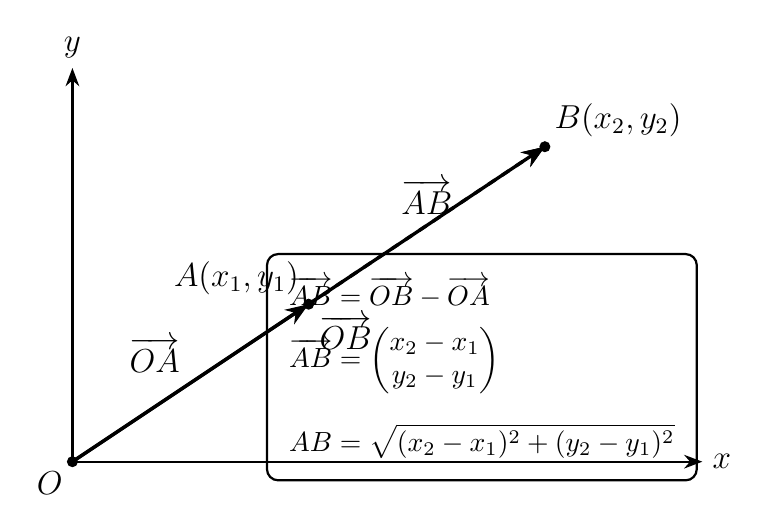
\begin{tikzpicture}[>=Stealth,axis/.style={->, thick},vector/.style={->, very thick},abvector/.style={->, very thick, dashed},label/.style={font=\large},formula/.style={draw, rounded corners, thick, align=left, inner sep=8pt}]
\draw[axis] (0,0) -- (8,0) node[right,label] {$x$};
\draw[axis] (0,0) -- (0,5) node[above,label] {$y$};
\coordinate (O) at (0,0); \coordinate (A) at (3,2); \coordinate (B) at (6,4);
\fill (O) circle (2pt) node[below left,label] {$O$}; \fill (A) circle (2pt) node[above left,label] {$A(x_1,y_1)$}; \fill (B) circle (2pt) node[above right,label] {$B(x_2,y_2)$};
\draw[vector] (O) -- (A) node[midway, above left,label] {$\overrightarrow{OA}$};
\draw[vector] (O) -- (B) node[midway, below right,label] {$\overrightarrow{OB}$};
\draw[abvector] (A) -- (B) node[midway, above,label] {$\overrightarrow{AB}$};
\node[formula] at (5.2,1.2) {$\displaystyle \overrightarrow{AB}=\overrightarrow{OB}-\overrightarrow{OA}$\\[6pt] $\displaystyle \overrightarrow{AB}=\begin{pmatrix}x_2-x_1\\y_2-y_1\end{pmatrix}$\\[10pt] $\displaystyle AB=\sqrt{(x_2-x_1)^2+(y_2-y_1)^2}$};
\end{tikzpicture}
\end{document}
